

\tikzset{every picture/.style={line width=0.75pt}} %set default line width to 0.75pt        

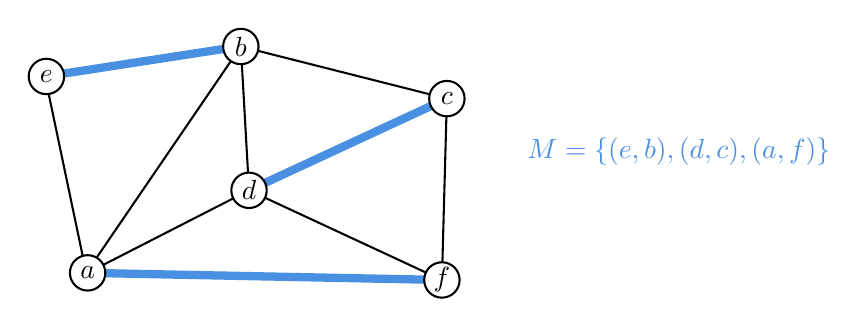
\begin{tikzpicture}[x=0.5pt,y=0.5pt,yscale=-1,xscale=1]
%uncomment if require: \path (0,202); %set diagram left start at 0, and has height of 202

%Straight Lines [id:da7485926733039977] 
\draw    (159.1,16.18) -- (47.37,179.77) ;
%Straight Lines [id:da4575120980127291] 
\draw [color={rgb, 255:red, 74; green, 144; blue, 226 }  ,draw opacity=1 ][line width=3]    (17.58,37.83) -- (158.1,16.18) ;
%Straight Lines [id:da9165715401778428] 
\draw    (17.58,37.83) -- (47.37,179.77) ;
%Straight Lines [id:da994182434786223] 
\draw [color={rgb, 255:red, 74; green, 144; blue, 226 }  ,draw opacity=1 ][line width=3]    (48.37,179.77) -- (304.41,184.9) ;
%Straight Lines [id:da9750224919648968] 
\draw    (165,120.11) -- (304.41,184.9) ;
%Straight Lines [id:da24348552449211425] 
\draw    (159.1,16.18) -- (165,120.11) ;
%Straight Lines [id:da16705340438790406] 
\draw    (159.1,16.18) -- (308,53.84) ;
%Straight Lines [id:da08663700279220432] 
\draw    (308,53.84) -- (304.41,184.9) ;
%Straight Lines [id:da16511775802360662] 
\draw [color={rgb, 255:red, 74; green, 144; blue, 226 }  ,draw opacity=1 ][line width=3]    (308,53.84) -- (165,120.11) ;
%Straight Lines [id:da4151454155794566] 
\draw    (165,120.11) -- (48.37,179.77) ;
%Shape: Ellipse [id:dp9133580928774087] 
\draw  [fill={rgb, 255:red, 255; green, 255; blue, 255 }  ,fill opacity=1 ] (5.79,37.83) .. controls (5.79,30.77) and (11.51,25.04) .. (18.58,25.04) .. controls (25.64,25.04) and (31.37,30.77) .. (31.37,37.83) .. controls (31.37,44.9) and (25.64,50.62) .. (18.58,50.62) .. controls (11.51,50.62) and (5.79,44.9) .. (5.79,37.83) -- cycle ;
%Shape: Ellipse [id:dp4005957609675306] 
\draw  [fill={rgb, 255:red, 255; green, 255; blue, 255 }  ,fill opacity=1 ] (146.31,16.18) .. controls (146.31,9.11) and (152.03,3.39) .. (159.1,3.39) .. controls (166.16,3.39) and (171.89,9.11) .. (171.89,16.18) .. controls (171.89,23.24) and (166.16,28.97) .. (159.1,28.97) .. controls (152.03,28.97) and (146.31,23.24) .. (146.31,16.18) -- cycle ;
%Shape: Ellipse [id:dp49214617921702164] 
\draw  [fill={rgb, 255:red, 255; green, 255; blue, 255 }  ,fill opacity=1 ] (295.21,53.84) .. controls (295.21,46.78) and (300.94,41.05) .. (308,41.05) .. controls (315.06,41.05) and (320.79,46.78) .. (320.79,53.84) .. controls (320.79,60.9) and (315.06,66.63) .. (308,66.63) .. controls (300.94,66.63) and (295.21,60.9) .. (295.21,53.84) -- cycle ;
%Shape: Ellipse [id:dp8440754424343925] 
\draw  [fill={rgb, 255:red, 255; green, 255; blue, 255 }  ,fill opacity=1 ] (152.21,120.11) .. controls (152.21,113.05) and (157.94,107.32) .. (165,107.32) .. controls (172.07,107.32) and (177.79,113.05) .. (177.79,120.11) .. controls (177.79,127.18) and (172.07,132.9) .. (165,132.9) .. controls (157.94,132.9) and (152.21,127.18) .. (152.21,120.11) -- cycle ;
%Shape: Ellipse [id:dp20660183368429152] 
\draw  [fill={rgb, 255:red, 255; green, 255; blue, 255 }  ,fill opacity=1 ] (35.58,179.77) .. controls (35.58,172.71) and (41.3,166.98) .. (48.37,166.98) .. controls (55.43,166.98) and (61.16,172.71) .. (61.16,179.77) .. controls (61.16,186.84) and (55.43,192.56) .. (48.37,192.56) .. controls (41.3,192.56) and (35.58,186.84) .. (35.58,179.77) -- cycle ;
%Shape: Ellipse [id:dp4098192910838151] 
\draw  [fill={rgb, 255:red, 255; green, 255; blue, 255 }  ,fill opacity=1 ] (291.62,184.9) .. controls (291.62,177.83) and (297.34,172.11) .. (304.41,172.11) .. controls (311.47,172.11) and (317.2,177.83) .. (317.2,184.9) .. controls (317.2,191.96) and (311.47,197.69) .. (304.41,197.69) .. controls (297.34,197.69) and (291.62,191.96) .. (291.62,184.9) -- cycle ;

% Text Node
\draw (18.58,37.83) node   [align=left] {$\displaystyle e$};
% Text Node
\draw (159.1,16.18) node   [align=left] {$\displaystyle b$};
% Text Node
\draw (308,53.84) node   [align=left] {$\displaystyle c$};
% Text Node
\draw (165,120.11) node   [align=left] {$\displaystyle d$};
% Text Node
\draw (48.37,179.77) node   [align=left] {$\displaystyle a$};
% Text Node
\draw (304.41,184.9) node   [align=left] {$\displaystyle f$};
% Text Node
\draw (364,80) node [anchor=north west][inner sep=0.75pt]   [align=left] {$\displaystyle \textcolor[rgb]{0.29,0.56,0.89}{M=\{( e,b) ,( d,c) ,( a,f)\}}$};


\end{tikzpicture}

